%   =============================================
%	Drawing uncompensated and compensated demands
%   following a price change
%   Author: Patrick Blanchenay
%   =============================================

\documentclass{standalone}
% =============================================
\usepackage{tikz}               % to draw things
\usetikzlibrary{intersections}  % to compute intersections automatically 
\usepackage{pgfplots}           % to draw plots & curves
\pgfplotsset{compat=1.8}
% =============================================
\begin{document}
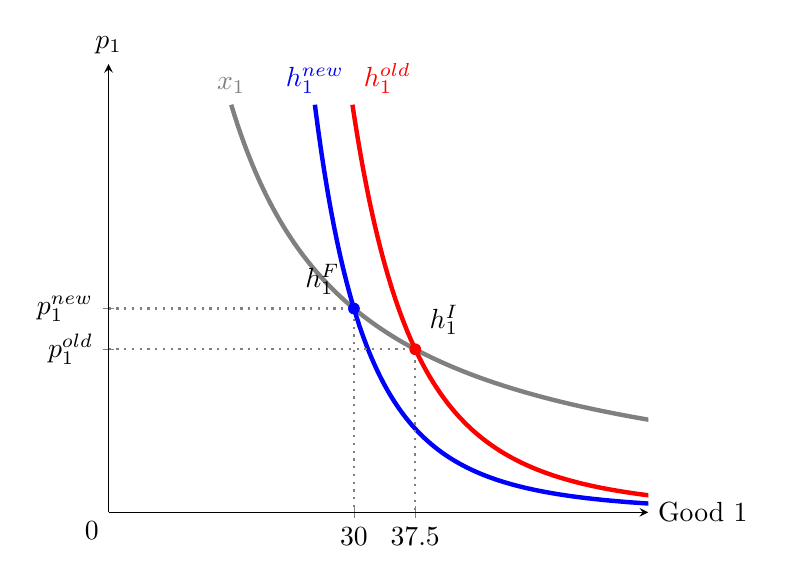
\begin{tikzpicture}
% ========= Things to change ======================
\def\hmax{60} \def\pmax{10} % maximum values for quantity and price on the graph (used to draw the axes)
\def\oldprice{4} % old price
\def\newprice{5} % new price
% ======= Compute those manually (p stands for the price p1)
\def\oldcompdemand{53.03*p^(-0.25)} % compensated demand under old utility level
\def\newcompdemand{44.86*p^(-0.25)} % compensated demand under new utility level
\def\uncompdemand{150/p} % uncompensated demand
\def\oldqtty{150/\oldprice} % demand at old price
\def\newqtty{150/\newprice} % demand at new price
% ======= GRAPH BEGINS HERE ===========
\begin{axis}[ 
 	axis lines=middle,
 	xlabel=Good $1$, xlabel style={right },
 	ylabel=$p_1$, ylabel style={above },
 	xmin=0,ymin=0,xmax=\hmax,ymax=\pmax,
 	enlarge y limits={upper=0.15},
 	enlarge x limits={upper=0.1},
 	xtick={0,\newqtty,\oldqtty}, % compute these manually
 	ytick={0,\oldprice,\newprice},yticklabels={0,$p_1^{old}$,$p_1^{new}$},
 	clip mode=individual, % clip plots to axes box but not text
 	]
% Axes origin
\node [below left] (origin) at (axis cs:0,0) {$0$};	

% uncomp demand x1
\addplot[name path global=x1uncomp,
samples=200,gray, ultra thick,domain=0.1:\pmax,variable=p] (\uncompdemand,p) node[above]{$x_1$};\textbf{}

% old h1 (lower samples means more jagged but faster to display)
\addplot[name path global=h1old,
	samples=200,red, ultra thick,domain=0.1:\pmax,variable=p] (\oldcompdemand,p) node[above right]{$h_1^{{old}}$};

% new h1 (lower samples means more jagged but faster to display)    
\addplot[name path global=h1new,
samples=200,blue, ultra thick,domain=0.1:\pmax,variable=p] (\newcompdemand,p) node[above]{$h_1^{{new}}$};

% Drawing the dots at the intersection (computed manually)
\path [name intersections={of=h1old and x1uncomp,by=i}]; % i: intersection of h1old and x1uncomp
\path [name intersections={of=h1new and x1uncomp,by=f}]; % f: intersection of h1new and x1uncomp
    
% Project intersections on the axes
\coordinate (verticalaxis) at (axis cs:0,\pmax); 
\coordinate (horizontalaxis) at (axis cs:\hmax,0); 
\draw[thick,gray,dotted] (f -| verticalaxis)  -- (f) -- (f |- horizontalaxis)  ; %
\draw[thick,gray,dotted] (i -| verticalaxis) -- (i) -- (i |- horizontalaxis) ; %

% Show and label the intersections
\node [fill=red,circle,inner sep=1.5pt,label= above right:$h_1^I$] at (i) {};
\node [fill=blue,circle,inner sep=1.5pt,label= above left:$h_1^F$] at (f) {};

\end{axis}
\end{tikzpicture}
% =============================================	
\end{document}